\documentclass{article}

\usepackage{tikz}
\usetikzlibrary{arrows}

\begin{document}

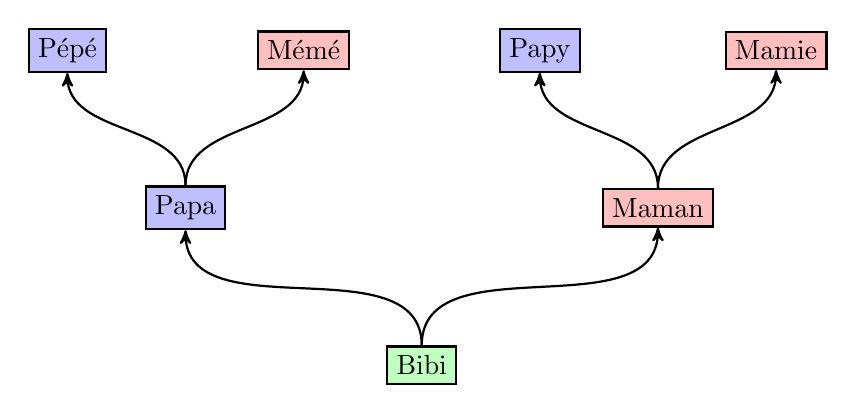
\begin{tikzpicture}[edge from parent path={[->,>=stealth',thick](\tikzparentnode) to [out=90,in=-90] (\tikzchildnode)}]
\tikzstyle{lien}=[->,>=stealth,rounded corners=5pt,thick]

\tikzset{individu/.style={draw,thick,fill=#1!25},individu/.default={green}}
\node [individu] {Bibi}[grow'=up,level distance=2cm,sibling distance=6cm]
child{
  node [individu=blue]{Papa} [sibling distance=3cm]
  child{node [individu=blue]{Pépé}}
  child{node [individu=red]{Mémé}}
}
child{
  node [individu=red]{Maman} [sibling distance=3cm]
  child{node [individu=blue]{Papy}}
  child{node [individu=red]{Mamie}}
};
\end{tikzpicture}


\end{document}
